\section{Path Discretisation}
The discrete approximation of the path was performed in order to solve for the time-optimal trajectory of the DoodleBot. The approximation of the problem spreads speed choking points of the path out over a greater path length, which intuitively leads to longer traversal times. The traversal time for a range of path discretisation divisions can be seen in Figure \ref{fig:sDivisions}. The overall trend for the traversal time is an exponential decay to a constant value which corresponds to the optimum traversal time for the true solution. This value is reached consistently at approximately 80 path divisions. As such, 80 divisions forms the lower bound on the number of discretisations for an acceptable approximation. As the number of control points increases, so too should the number of discretisations, as the number of control points a curve contains correlates linearly with the complexity of the curve and linearly with the number of possible limiting axis switching points.

An interesting effect and something that showcases a flaw in the discretisation approximation can also be seen in Figure \ref{fig:sDivisions}. Note the repetitive stutter pattern in the shape of the decaying completion time. Note also, that the completion time for some of the stutters falls below the convergent minimum possible value. This effect is caused by the path discretisation approximating the constraints of the curve as though the system can be traversed faster than the true constraints allow. This occurs due to the discrete switching of the restrictions extending a section that allows fast travel for longer than that section actually exists. This extension exists even though maximums are taken of the magnitude of the path derivatives, as discussed in previous sections. The combinations of the signs and magnitudes of the path derivatives mean that something that the algorithm picks as a constraint, might not actually be the true constraint for the entire discretisation. This bleeding specifies that the DoodleBot should be speeding up when, in order to obey the constraints, it should be slowing down. Thus a lower number of path divisions may result in a trajectory which is impossible for a mechanism with the limits on acceleration specified to traverse. This effect is possible at 80 path divisions and even higher, but is can be seen from the decaying oscillation that the effect becomes a smaller problem at higher divisions. The effect is also mitigated by the fact that the hard limits of the motor are not the limits that are set for the solution, but rather a smaller soft limit is requested. This allows the small trespasses on the maximum limits to be followed by the motors without error.


\begin{figure}[htbp]  
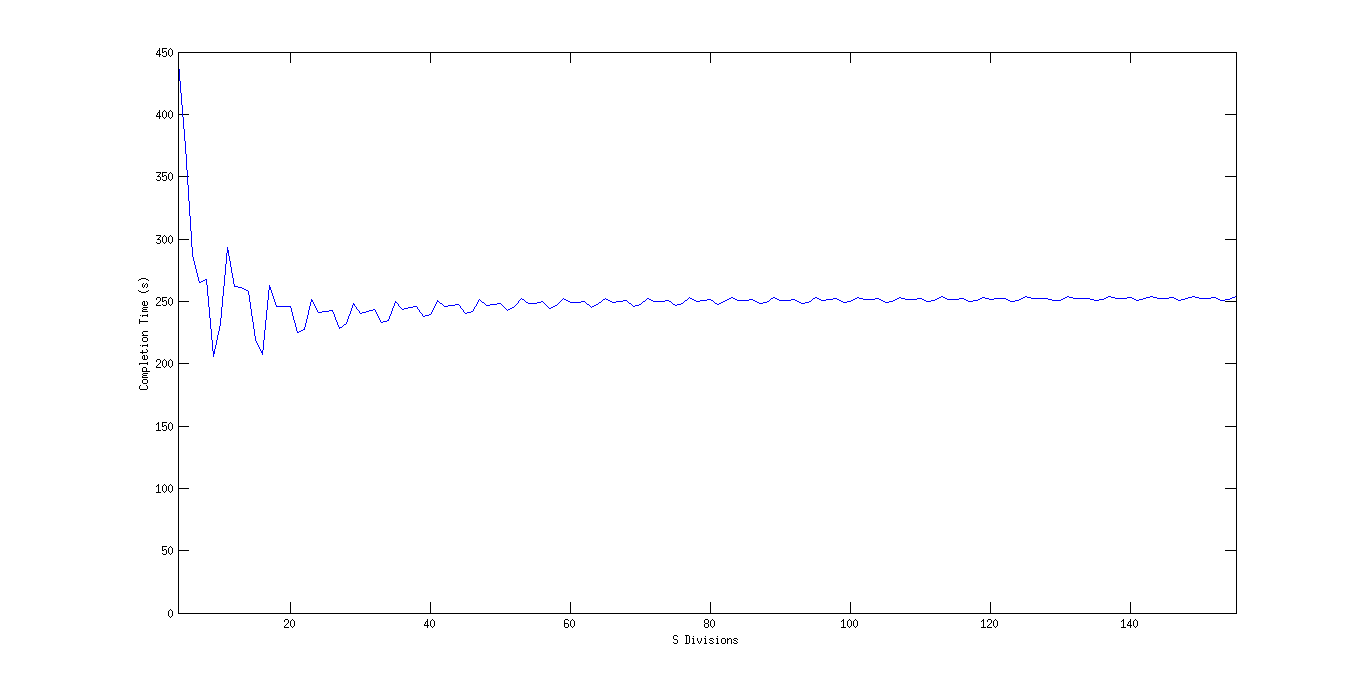
\includegraphics[width=\textwidth]{figures/performance/sDivisions.png}
\caption[Trajectory completion time for a range of path discretisation divisions]{Trajectory completion times for a range of path discretisation divisions
\label{fig:sDivisions}}
\end{figure} 

A limitation of the solution process that prevents the solver from simply solving for an arbitrarily large number of discretisation steps is the fact that the solver becomes numerically unstable at a threshold of around 1500 discretisation intervals, meaning that solutions are often not possible past this value. A second reason which forms a limitation when one considers the desire to minimise the length of the whole printing process is the exponential growth of computation time as the number of discretisation intervals increases. The DoodleBot processes the input upon the request of the user to print a series of curves. Ideally, the processing time of the curve optimisation is not the limiting factor in the printing process. However with large discretisation values, the processing time balloons out to values such as 384 seconds, or about 6 minutes per curve. This means that a tradeoff between the computation time and optimality must be made. Figure \ref{fig:sDivTime} demonstrates the processing time increase with the number of divisions. The average traversal time for a curve on the DoodleBot hardware is about 8 seconds at the optimal torque limits. This approximately corresponds the value that was set for the DoodleBot's default number of path discretisations, at 200. This level of discretisation gives a good approximation of the optimal solution without stretching the acceleration constraints. This value also remains below the average curve execution time, so that curves are processed faster than they are traversed.

\begin{figure}[htbp]  
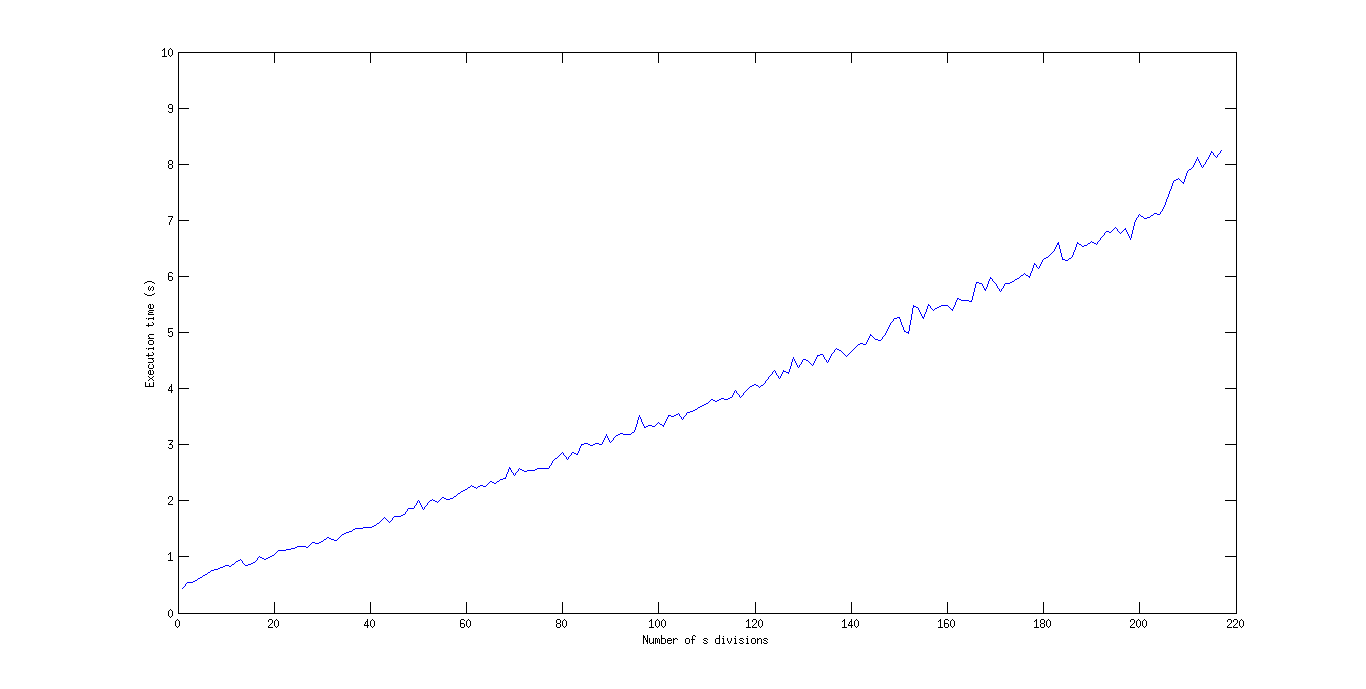
\includegraphics[width=\textwidth]{figures/performance/sDivTime.png}
\caption[Processing time for a range of path discretisation divisions]{Processing time for a range of path discretisation divisions
\label{fig:sDivTime}}
\end{figure} 


